\section{Page--Wootters and detector absorption models}\label{sec:absorption+pw}

The detector absoption model in \cite{RuschhauptAbsorption} is not originally
based on the notion of quantum relational time. It's ``ordinary quantum mechanics''
in the sense that states are in $\hilb{H}_S$ with an external parameter time;
but, contrary to quantum mechanics, the potential can be \emph{complex},
causing the norm of the state vector to not be conserved (in fact, vanishing with time).
In other terms, the evolution is not unitary, even for a pure state.
Specifically, the Hamiltonian is corrected by an anti-hermitian term
that models the detector.

A non hermitian Hamiltonian is justified as a computation method
to simplify the study of some open systems: the evolution of mixed
states is derived without explicit reference to density operators
or master equations, but resolving equations that are formally
identical to those of pure states,
i.e. in terms of
Schr{\"o}dinger equations and wave functions,
with the non-hermitian term in the Hamiltonian
to account for the non-unitarity of the evolution.
%
This is treated extensively in
  \cite{Wave-function_approach, HowToResetAnAtom, TheQuantumJumpApproach};
in
  \cite[Ch. 6]{TQM2};
in
  \cite[\S 8.5.2 ``The `quantum jump' approach to damping: The wave function Monte Carlo approach'']{ScullyZubairy};
and in
  \cite[\S 6.7.1 ``Simulating Quantum Trajectories'']{WallsMilburn}.

The detection-by-absoption model in \cite{RuschhauptAbsorption}
is based on a complex potential that, plugged into the Schr\"odinger equation,
leads to a non-unitary evolution of the state vector
(with loss of normalization).

Specifically, the Hamiltonian $\hat{H}$ is replaced by a $\hat{H} - i\hat{D}$
(with $\hat{D}$ self-adjoint, bounded, positive)
and, consequently:
\begin{equation}\label{eq:schrod_complex_pot}
  \hat{H} \ket{\psi(t)} = i\hbar\dv{t}\ket{\psi(t)} +i\hat{D}\ket{\psi(t)} \text{.}
\end{equation}

One may wonder whether a proper, normalized Page--Wootters ``position-time wavepacket''
(as described in Section \ref{sec:properpw})
can be used to describe \emph{the event of being detected} (or being absorbed).
It's expected to be peaked around the time when the absorption by the detector is maximum.

In the detector model of \cite{RuschhauptAbsorption}, the detection
by absorption
corresponds to the \emph{decrease} in norm of the wavefunction.

Therefore we expect the following relation to be true:
\begin{equation}\label{eq:pwkiukas}
  \braket{\phi(t)} = -\dv{t}\norm{\psi_{\text{Kiukas}}(t)}^2 \text{,}
\end{equation}
both sides of which indicate probability of arrival at time $t$.
Here the function $\phi$ of time $t$ has to be intended in the sense of
\eqref{eq:pwphi}.

Interestingly, \cite{RuschhauptAbsorption} provides a solution of \eqref{eq:pwkiukas}.
Despite being not based on the Page--Wootters model, eq. 9 therein
equates the squared norm of a ``time representation'' wavefunction
to the opposite derivative of the squared norm of the ``absorbed wavefunction''.
It reads:
\begin{quote}
  We will associate with any wave function $\psi \in \hilb{H}$
  another wave function $\hat{\psi}$,
  which is a function of time, so that
  $\abs{\hat{\psi}(t)}^2$
  is the arrival probability density. In other words,
  $\hat{\psi}$ is a wave function in a time representation. For each
  $t$, $\hat{\psi}(t)$ lies in the original Hilbert space $H$.
\end{quote}
Therefore we ``translate'' $\hat{\psi}(t)$ into $\ket{\phi(t)}_S$
and, consequently, $\abs{\hat{\psi}(t)}^2$ into $\braket{\phi(t)}$,
in the language of the Page--Wootters model and within the notation
adopted.

Using eq. 8 in \cite{RuschhauptAbsorption} and translating into our notation we have:
\begin{equation}\label{eq:phi_psi_kiukas}
  \hat{\psi}(t) \eqbydef
  \ket{\phi(t)}_S =
  \begin{cases}
    \sqrt{\frac{2}{\hbar}} \hat{D}^{1/2} \ket{\psi_{\text{Kiukas}}(t)}_S &\text{ if } t > 0 \\
    0 &\text{ otherwise. }
  \end{cases}
\end{equation}
Where at $t \le 0$ the interaction with the detector is yet to come,
but so it is, as a limit, for small values of $t>0$,
in other terms
$\lim_{t \to 0^{+}} \norm{\hat{D} \ket{\psi_{\text{Kiukas}}(t)}} = 0$, thus avoiding the apparent discontinuity.

% \subsection*{\color{red} TODO}

% {
%   \color{red}
%   Figure out how to connect the above to what follows (or drop or separate if does not apply).

%   \scriptsize{
%     Hint: rather then the ``conspiracy theory''
%     (``I find an imaginary term both here and there'')
%     consider (time of) arrival as in \cite{Maccone:QMOT}.
%     This should bring to a normalized element of $\pwspace$ \dots
%   }
% }

\subsection{Application: two-level system}

In \cite{RuschhauptAbsorption}, an example application of the detector model
is provided for a two-level system.
In Page and Wootters terms,
this would corrspond to a bi-dimensional $\hilb{H}_S$, but a continuous
spectrum of $\hat{T}$ in $\hilb{H}_T$. The paper is \emph{not} based on
the Page--Wootters model, indeed the purpose of this section is a comparison
with such model, using the results of Section \ref{sec:absorption+pw}.

By setting, out of convenience, $\hbar = \omega = 1$
(with $\omega$ the characteristic frequency of the system),
and directly considering the parameters
that minimize the time--energy uncertainty product \parencite{RuschhauptAbsorption},
we have a non-Hermitian ``Hamiltonian''
$\mathit{K} = \hat{H} - i\hat{D}$ with
\begin{equation}\label{eq:complexpot}
  \mathit{K} = \hat{H} - i\hat{D} \repr
    \hbar\omega\left\{
      \left[\begin{matrix}0 & 1\\1 & 0\end{matrix}\right] -
      i \left[\begin{matrix}0 & 0\\0 & \gamma \end{matrix}\right]
    \right\}
\end{equation}
and $\gamma = 2\sqrt{2}$.

We take an initial state of $\ket{0}$
(or $\mqty[1\\0]$ in matrix form).

We then compute, symbolically, the non-unitary evolution
$\ket{\psi(t)} = e^{-i\mathit{K}t}\ket{0}$
with the aid of \term{SymPy} \parencite{comp:sympy} within a \term{Jupyter} \parencite{comp:jupyter} notebook
(see Appendix \ref{detector-model-kiukas-ruschhaupt-schmidt-werner} for all the details of the calculation).

Simplifying the result in eq. \eqref{eq:sympy:non-unitary-evol}, we have:
\begin{equation}
  \ket{\psi(t)} \repr e^{-\frac{\sqrt{2}}{t}} \mqty[
    \cos(\frac{\sqrt{2}}{2}t) + \sin(\frac{\sqrt{2}}{2}t)& \\
                     -i\sqrt{2} \sin(\frac{\sqrt{2}}{2}t)&
  ] \,\text{.}
\end{equation}

\begin{figure} %% https://tex.stackexchange.com/a/165730
  \centering
  \begin{subfigure}{0.49\textwidth}
    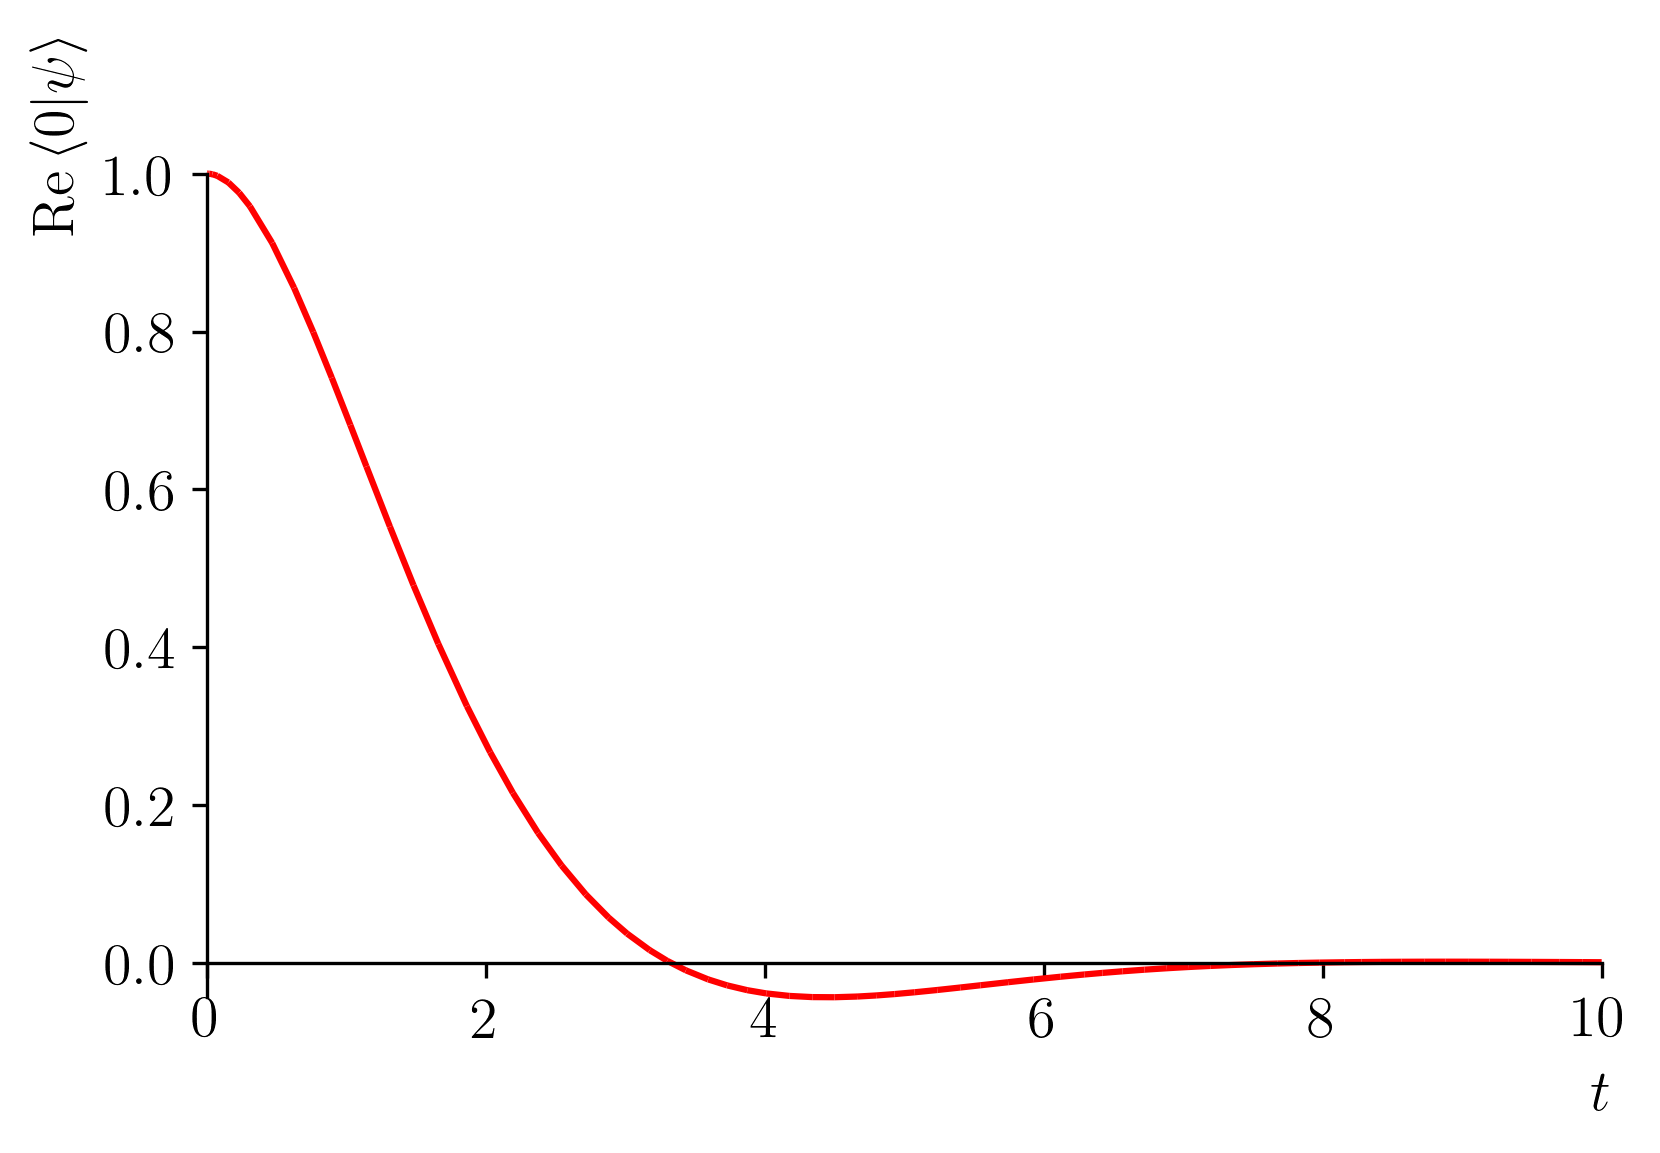
\includegraphics[width=\linewidth]{img/2ldetect/re_psi0_t.png}
    \subcaption{}\label{fig:absorbed-qubit-components:re0}
  \end{subfigure}
  % \hspace*{\fill} % separation between the subfigures
  \begin{subfigure}{0.49\textwidth}
    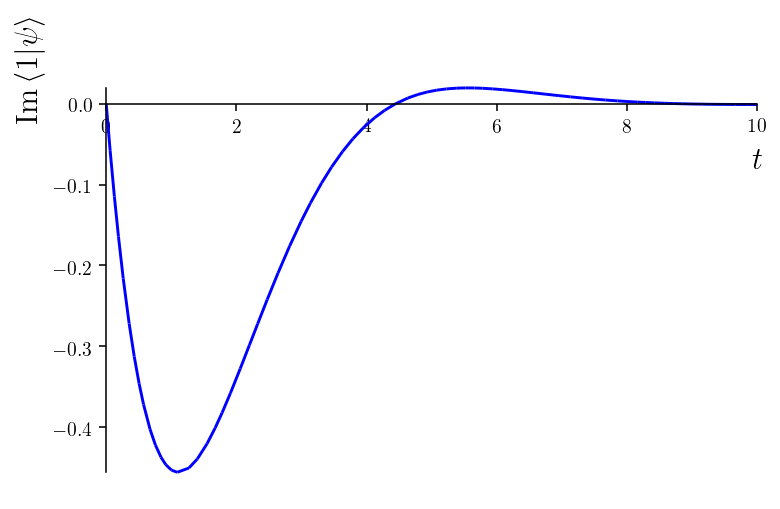
\includegraphics[width=\linewidth]{img/2ldetect/im_psi1_t.png}
    \subcaption{}\label{fig:absorbed-qubit-components:im1}
  \end{subfigure}
  % \hspace*{\fill} % separation between the subfigures
  \caption{
    Non-unitary evolution of the absorbed qubit
    according to the model in
    ref. \cite[\S ``Emission from a two-level system'']{RuschhauptAbsorption}.
    The component along $\ket{0}$ is purely real,
    and the one along $\ket{1}$ is purely imaginary,
    therefore only their their respective parts are plotted.
  }\label{fig:absorbed-qubit-components}
\end{figure}

\begin{figure}
  \centering
  \begin{subfigure}[b]{0.49\textwidth}
    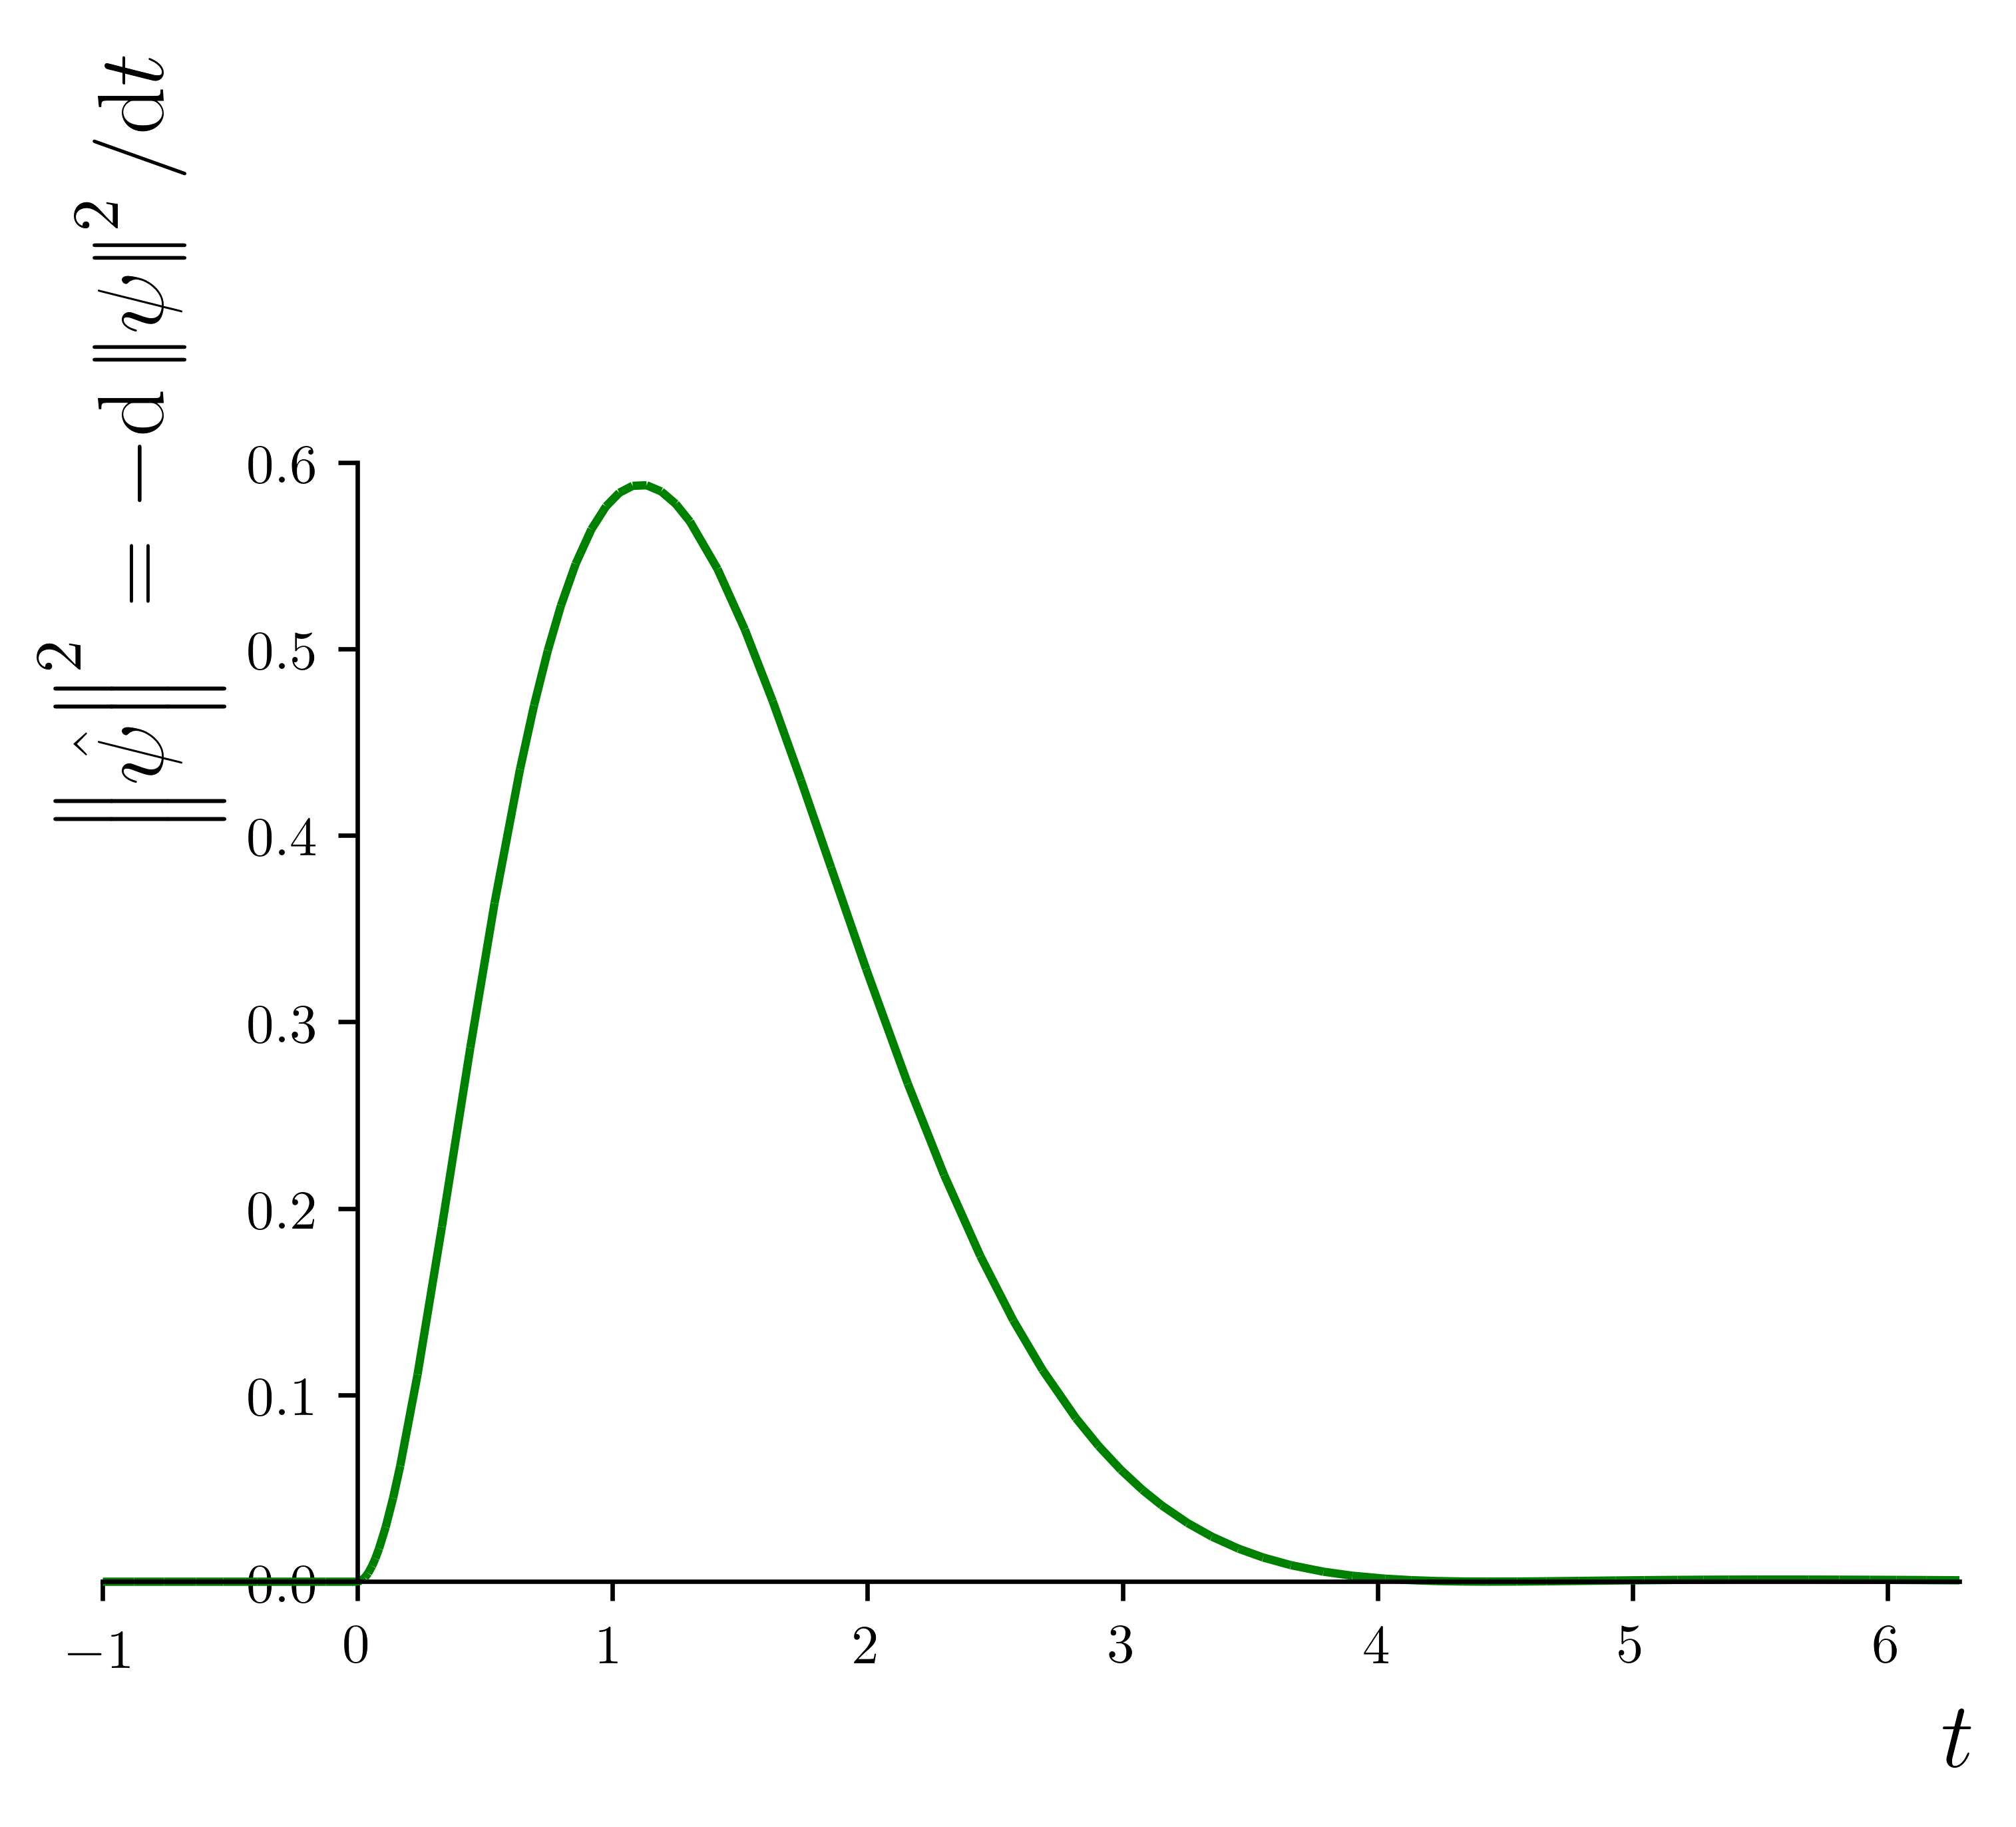
\includegraphics[width=\linewidth]{img/2ldetect/qubit_normalization_loss.png}
    \subcaption{}\label{fig:absorbed-qubit-normalization-loss:t}
  \end{subfigure}
  \begin{subfigure}[b]{0.49\textwidth}
    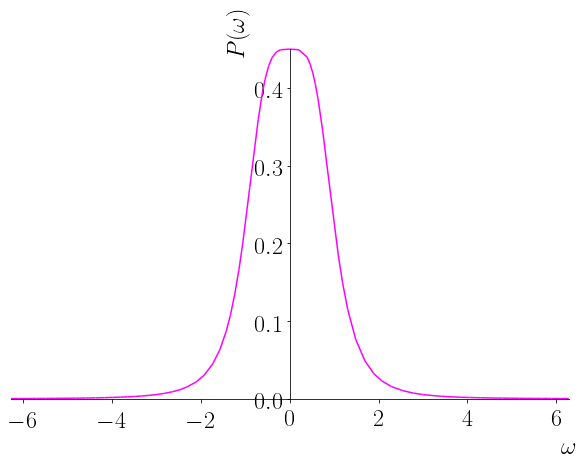
\includegraphics[width=\linewidth]{img/2ldetect/P_omega.png}
    \subcaption{}\label{fig:absorbed-qubit-normalization-loss:omega}
  \end{subfigure}
  \caption{
    Non-unitary evolution of absorbed qubit.
    \subref{fig:absorbed-qubit-normalization-loss:t}
      Detection probability in time. It's equal to the
      loss of normalization $-\dv{\norm{\psi}^2}{t}$
      (but also to the squared norm of $\hat{\psi}(t)$ as of eq. \eqref{eq:analytic:hatpsi}.
    \subref{fig:absorbed-qubit-normalization-loss:omega}
      Detection probability in the frequency domain.
  }
  \label{fig:absorbed-qubit-normalization-loss}
\end{figure}

The ``lossy'' evolution, with the two components of the qubit, is shown in Fig.~\ref{fig:absorbed-qubit-components}.
The loss of normalization $-\dv{\norm{\psi}^2}{t}$, indicating the probability of detection by absorption,
is then derived directly and shown in Fig.~\ref{fig:absorbed-qubit-normalization-loss}.

This yields the \emph{probability} of detection.
One may wonder whether it is possible to derive a corresponding \emph{probability amplitude} vector,
whose squared norm across time is equal to the said probability distribution.\footnote{
  The solution is of course not unique, but one may ask whether such functions would lead
  to quantum interference patterns and other phenomenology which may be subject of further study.
}
Within the framework of \cite{RuschhauptAbsorption}, a ``wavefunction in time'' in such sense
is the $\hat{\psi}$, as in \eqref{eq:phi_psi_kiukas}.
It is computed in detail within the
notebook in Appendix \ref{detector-model-kiukas-ruschhaupt-schmidt-werner}, eq. \eqref{eq:sympy:hatpsi},
simplifying which we obtain:
\begin{equation}\label{eq:analytic:hatpsi}
  \hat{\psi}(t) =
    i 2^{\frac{5}{4}} e^{-\frac{\sqrt{2}}{2}t}\sin(\frac{\sqrt{2}}{2}t) \theta(t)
    \ket{1}
    \text{,}
\end{equation}
with $\theta(t)$ the Heaviside step function.

\begin{remark}\label{remark:detection_area}
In general, the operator $\hat{D}$ as in \eqref{eq:schrod_complex_pot}
is such that the eigenspace corresponding to its zero eigenvalue
is the ``area'' where the detector is not sensitive. Or, in other words,
the linear span of states with zero probability of triggering the detector.
Therefore, when $\hat{D}$ (or its square root) is applied to a state vector,
for example in \eqref{eq:phi_psi_kiukas},
the components in such eigenspace are cut off and the resulting
$\hat{\psi}$, eq. \eqref{eq:analytic:hatpsi} in the example, lies at all times in the ``area of detection''
i.e. it's a multiple of $\ket{1}$ in this case.
\end{remark}

The corresponding Page--Wootters (proper) vector of $\pwspace$ is
\begin{equation}\label{eq:hatpsi:pw}
  \dket{\Phi} = \int \dd{t} \ket{t} \ox \hat{\psi}(t) \,\text{,}
\end{equation}
to which the considerations of Section \ref{sec:for-normalized-elements}
and Section \ref{sec:pure-state-approach} in terms of time--frequency
(or time--energy) uncertainty relation apply, with some analogy
to what \cite{RuschhauptAbsorption} does within its own framework
in relation to $\hat{\psi}$ and its Fourier transform.

In that regard, the \eqref{eq:hatpsi:pw} can be reformulated
\begin{equation}
  \dket{\Phi} = \int \dd{\omega} \ket{\omega} \ox \mathcal{F} \hat{\psi} (\omega) \,\text{,}
\end{equation}
where it's
\begin{equation}
  \mathcal{F} \hat{\psi} (\omega) = - \frac{\sqrt[4]{2} i}{\sqrt{\pi} \left(- \omega^{2} + \sqrt{2} i \omega + 1\right)} \ket{1}
\end{equation}
---see notebook up to eq. \eqref{eq:fhatpsi1_omega} for details.

Taking the squared modulus, a probability distribution over angular frequency
(or, equivalently, energy) is obtained:
\[
  P(\omega) = \frac{\sqrt{2}}{\pi \left(\omega^{4} + 1\right)}
  \,\text{.}
\]
See Fig. \ref{fig:absorbed-qubit-normalization-loss:omega}.

\subsubsection{
  (Non-unitary) evolution without evolution:
  plugging the complex potential in the \emph{discrete} Page--Wootters model
}

Similarly to what seen in Section \ref{sec:building-the-discrete-pw-clock}, we build
the clock by defining ---and representing in a convenient basis---
the time operator and the corresponding frequency operator:
\begin{align}
  \hat{T} \repr \frac{2\pi}{N}
  \begin{pmatrix}
    0           &       &       &       \\
                &1      &       &       \\
                &       &\ddots &       \\
                &       &       &N-1
  \end{pmatrix}
  &&
  \hat{\Omega} = \frac{N}{2\pi} F^{}_{N} \hat{T} F^{\dagger}_{N} \, \text{,}
\end{align}
where $F$ is, again, the discrete Fourier operator of order $N$.

Next we define the Wheeler--DeWitt operator $\mathbb{J}$ as in
\eqref{eq:pwHamiltonian}, but $\hat{H}_S$ is replaced by the non-hermitian
Hamiltonian of the detector model
$\mathit{K}_S = \hat{H}_S - \iu \hat{D}_S$
\parencite{RuschhauptAbsorption},
where the subscript $_S$ has been added to stress
that they would act on the $\hilb{H}_S$ part
of the Page--Wootters' $\pwspace$ ``spacetime'':
\begin{equation}
  \mathbb{J} = \hbar\hat{\Omega}\ox\idop_S + \idop_T\ox\qty(\hat{H}_S -\iu \hat{D}_S) \,\text{.}
\end{equation}
$\hat{H}_S$ and $\hat{D}_S$ are the same as $\hat{H}$ and $\hat{D}$
respectively from the \eqref{eq:complexpot}.

We then compute eigenvalues and eigenvectors of $\mathbb{J}$.
Eigenvectors associated to the eigenvalue $0$ will include
the history of the qubit over a ``period''
(of what would have been a periodic evolution, without the absorptive detector).

Eigenvectors associated to non-zero eigenvalues will need a ``phase correction'',
or energy shift\footnote{ Again, see also ref. \cite[\S ``The Zero-eigenvalue'']{Lloyd:Time}. }
as seen, for example, in \eqref{eq:comparison0} and \eqref{eq:comparison1}.
Or, in a more compact form:
\begin{equation}
  \dket{n}_{\text{hist.}} = e^{-\iu \epsilon_n \hat{T}} \ox \idop_S \dket{n}
  \,\text{,}
\end{equation}
where $\epsilon_n$'s are eigenalues of $\mathbb{J}$ and
$\dket{n}$'s their corresponding eigenvectors.

Linear combination of histories $\sum_n \alpha_n \dket{n}_{\text{hist.}}$
are also physically possible\footnote{
  As opposed to (linear combinations of) mere, uncorrected eigenstates of $\mathbb{J}$.
  Indeed, one may observe,
  at least in the case where $\mathbb{J}$ was hermitian,
  that $\setof{\dket{n}}$ is a basis
  of $\pwspace$ therefore
  $\sum_n \alpha_n \dket{n}$ would span \emph{all elements}
  of $\pwspace$ and the theory would not predict anything i.e.
  it would not discriminate unphysical histories.
}
and in fact we pick
one that ensure that the initial state ${}_{T}\bradket{0}{\Psi}$ is equal to $\ket{0}_S$
so to allow a comparison with the example in \cite{RuschhauptAbsorption}.
Such linear combination is not unique. For reasons of numerical stability,
a linear combination with coefficients in the order of 1 would be ideal if it exists.
In this particular problem, it does.
We simply scan, as a first attempt, all possible values ${}_{T}\bradket{0}{n} + {}_{T}\bradket{0}{m}$
to find a combination that is equal to $\ket{0}_S$
-- or maximizes the fidelity with that respect.\footnote{
  See the definition, and invocation, of the function \texttt{find_best()} in Appendix \ref{discrete-page-wootters-model}.
}

All the above numerical computation is implemented with \emph{NumPy} \parencite{comp:numpy},
particularly in appendix
\S \ref{discrete-page-wootters-model}.
The results are visualized in
Fig. \ref{fig:absorbed-qubit-components_pwlattice},
and are \emph{compatible} with the non-Page--Wootters
solution previously shown in Fig. \ref{fig:absorbed-qubit-components}.

\begin{figure}
  \centering
  \begin{subfigure}[b]{0.49\textwidth}
    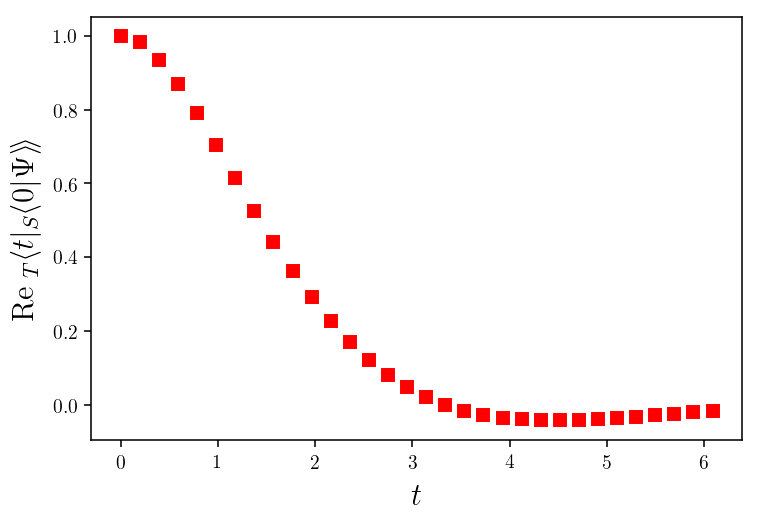
\includegraphics[width=\linewidth]{img/2ldetect/re_psi0_t_pwlattice.png}
    \subcaption{}\label{fig:absorbed-qubit-components_pwlattice:re0}
  \end{subfigure}
  \begin{subfigure}[b]{0.49\textwidth}
    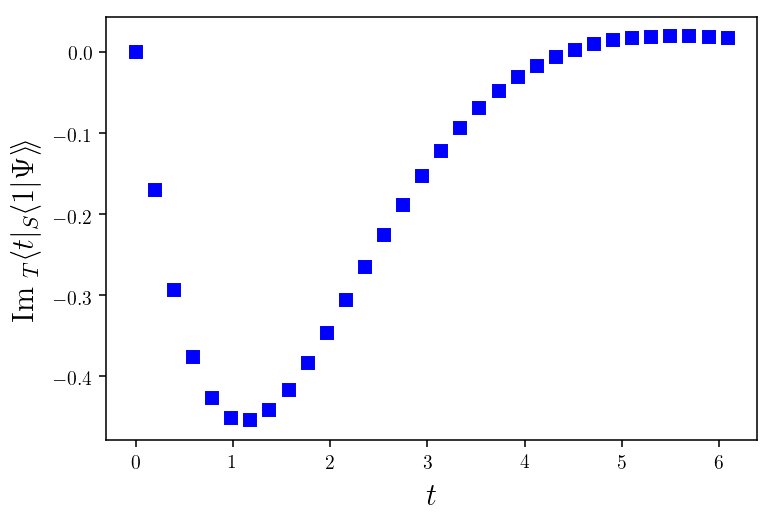
\includegraphics[width=\linewidth]{img/2ldetect/im_psi1_t_pwlattice.png}
    \subcaption{}\label{fig:absorbed-qubit-components_pwlattice:im1}
  \end{subfigure}
  \caption{
    Non-unitary ``evolution without evolution''
    using the discrete Page--Wootters model,
    plugging in
    the complex potential of \cite{RuschhauptAbsorption}.
    The result is compatible with the continuous
    ``Schr\"odinger evolution''
    shown in Fig. \ref{fig:absorbed-qubit-components}.
    Note the different notation e.g.
    $\mathrm{Re}{\;}_{T}\hspace{-.2em}\left\langle t | {}_{S}\hspace{-.2em}\left\langle 0 | \Psi \right\rangle\hspace{-.17em}\right\rangle$
    to fit within the framework of the P--W space-time $\pwspace$.
  }
  \label{fig:absorbed-qubit-components_pwlattice}
\end{figure}

\subsubsection{Detection probability amplitude, time of arrival distribution}

In \cite{RuschhauptAbsorption} the probaility of detection in time is given
by how fast the norm decreases i.e. $-\dv{\norm{\psi}^2}{t}$.
A ``wavefunction in time'', whose squared modulus equates the detection probability,
is introduced in eq. (8) therein:\footnote{
  Please note we are importing some notation from \cite{RuschhauptAbsorption} as per the symbol $\hat{\psi}$,
  at variance to what generally adhered to in this work,
  where the ``hat'' ($\hat{\;}$) denotes quantum observables and their corresponding operators.
}
\begin{equation}
  \hat{\psi} = \theta(t) \sqrt{2/\hbar}\,\hat{D}^{1/2}\,\psi
\end{equation}
In Page--Wooters terms, this translates into applying
$\theta(\hat{T}) \ox \sqrt{2/\hbar}\,\hat{D}^{1/2}_S$
to the each history vector $\dket{n}_{\text{hist.}}$
(and their linear combinations).
The result is a detection-event \emph{proper} element of ${\pwspace}$
(that would be normalizable in a continuous, infinite-time model too):
\begin{equation}\label{eq:qubit_detection_wavefunction}
  \dket{\Phi_n} =
    \theta(\hat{T}) \ox \sqrt{2/\hbar}\,\hat{D}^{1/2}_S \dket{n}_{\text{hist.}} =
    \theta(\hat{T}) e^{-i\epsilon_{n}\hat{T}} \ox \sqrt{2\hat{D}} \dket{n} \, \text{.}
\end{equation}
Given we are considering, in our discrete model, only an interval of time within $0$ and $2\pi$,
i.e. all non-negative times (or, more physically, only times when the detector is active),
the Heaviside function $\theta$ (of operator) can be omitted, and simply replaced
by the identity in time $\idop_T$.

Of course, for our problem, we take a linear combination
\begin{equation}
  \dket{\Phi} = \sum_n \alpha_n \dket{\Phi_n}
\end{equation}
where the coefficients $\alpha_n$ are the same that verified
(not necessarily uniquely)
the initial condition of the problem
$\ket{0}_S = {}_T\bradket{0}{\Psi} = \sum_n \alpha_n \, {}_T\bradket{0}{n}_{\text{hist.}} = \sum_n \alpha_n \, {}_T\bradket{0}{n}$.

The vector $\dket{\Phi}$, proper element of $\pwspace$,
is the Page--Wootters counterpart of the function
``in time representation'' $\hat{\psi}$,
as
described in \cite{RuschhauptAbsorption}. In formulas:
\begin{equation}
  \bradket{t}{\Phi} = \hat{\psi}(t) \, \text{.}
\end{equation}

As a consequence of Remark \ref{remark:detection_area},
the ``detection wavefunction''~$\dket{\Phi}$ will always lie,
\emph{spatially},
in the space generated by $\ket{1}_S$, or in other terms:
\begin{equation}\label{eq:detect_prob_ampl_only_on_1}
  \prescript{}{T}{\bra{t}}\prescript{}{S}{\bradket{0}{\Phi}} = 0 \text{,} \quad \forall t \, \text{.}
\end{equation}
The linear space of $\ket{1}_S$ is the ``detectable area'' of the qubit
in this problem, and
$\dket{\Phi}$ is essentially the result of the action of the operator $\hat{D}$,
that filters non-detectable components out from any vector of $\hilb{H}_S$.

We derive the components of $\dket{\Phi}$ numerically in Section \ref{detection-event},
where they are encoded in the array \texttt{prob_detect_v}.
We observe therein that the \eqref{eq:detect_prob_ampl_only_on_1} is confirmed,
and that ${}_T\!\bra{t} {}_S\!\bradket{1}{\Phi}$ is proportional
to the $\ket{1}$-component of the evolution of the qubit (history $\Dket{\Psi}$)
at any time $t$
(%
  which is not surprising, being $\sqrt{2/\hbar}\hat{D}^{1/2}$ of the form
  $\scriptsize \left[\begin{matrix}0 & 0\\0 & \kappa \end{matrix}\right]$%
).
In more formal terms:
\begin{equation}\label{eq:detect_prob_amplitude_proportional}
  \exists \kappa: \: {}_T\!\bra{t} {}_S\!\bradket{1}{\Phi} = \kappa \cdot {}_T\!\bra{t} {}_S\!\bradket{1}{\Psi} \; \forall t \text{,}
\end{equation}
which, algbebraically, is almost obvious, given the considerations above.
However, it's worth noting that the expression on the right side
(up to a factor $\kappa$) is, at each $t$,
an ordinary quantum mechanical probability amplitude
(probability amplitude of being $\ket{1}$ rather than $\ket{0}$);
while the expression on the left side, as a function of $t$,
is a probability amplitude \emph{in time}.
Even when normalized (in the probabilistic sense), the two expressions
are proportional but not equal (hence the factor $\kappa$).
This is because the expression on the right must be normalized
so that, at each $t$,
${ \abs{ {}_T\!\bra{t} {}_S\!\bradket{0}{\Psi} }^2 + \abs{ {}_T\!\bra{t} {}_S\!\bradket{1}{\Psi} }^2 = 1 }$
(or, actually, equal to $ \braket{\psi(t)} \leq 1$, the ``lossy norm'' due to absorption).
Whereas the expression on the left must be normalized so that
$\sum_t \norm{ {}_T\!\bradket{t}{\Phi} }_S^2 = P$,
where $P$ is the total probability that the detection/absorption happens at any time,
and it's equal to $1$ for an ideal detection.

The probability of detection in time is shown in Fig. \ref{fig:2l_pw_detect_prob_t}
and is \emph{consistent} with the result of
the contuinuous and not explicitly Page--Wooters model of
\cite{RuschhauptAbsorption} (see Fig. \ref{fig:absorbed-qubit-normalization-loss:t}).

Switching to the frequency (and, therefore, \emph{energy}) domain,
the discrete Fourier transform yields another proper vector
$\Dket{\tilde{\Phi}}$ of $\pwspace$:
\begin{equation}
  \Dket{\tilde{\Phi}} = F \ox \idop_s \dket{\Phi} \, \text{.}
\end{equation}
This vector numerical values, taken pairwise
(or by groups of 3 for a qutrit etc.)
are the components in the computational basis
of the kets $\ket{\tilde{\phi}(\omega)} \in \hilb{H}_S$
such that
\begin{equation}
  \dket{\Phi} = \sum_n \ket{t}\bradket{t}{\Phi} = \sum_{\omega} \ket{\omega}\bradket{\omega}{\Phi}
    = \sum_{\omega} \ket{\omega}_T \ox \ket{\tilde{\phi}(\omega)}_S \, \text{.}
\end{equation}

As a numerical array, $\Dket{\tilde{\Phi}}$ is the representation of $\Dket{\Phi}$
under the basis $\ket{\omega} \ox \ket{0,1}$ instead of $\ket{t} \ox \ket{0,1}$,
where the $\ket{\omega}$ constitute an eigenbasis of angular frequency $\hat{\Omega}$.

The squared norms $\braket{\tilde{\phi}(\omega)}_{\!S} = \norm{\braDket{\omega}{\Phi}}_S^2$
give the probability of detection in the frequency domain, which is plotted in
Fig. \ref{fig:2l_pw_detect_prob_omega} and, again, consistent
with Fig. \ref{fig:absorbed-qubit-normalization-loss:omega} i.e.
the result from the model of \cite{RuschhauptAbsorption}.

\begin{figure}
  \centering
  \begin{subfigure}[b]{0.49\textwidth}
    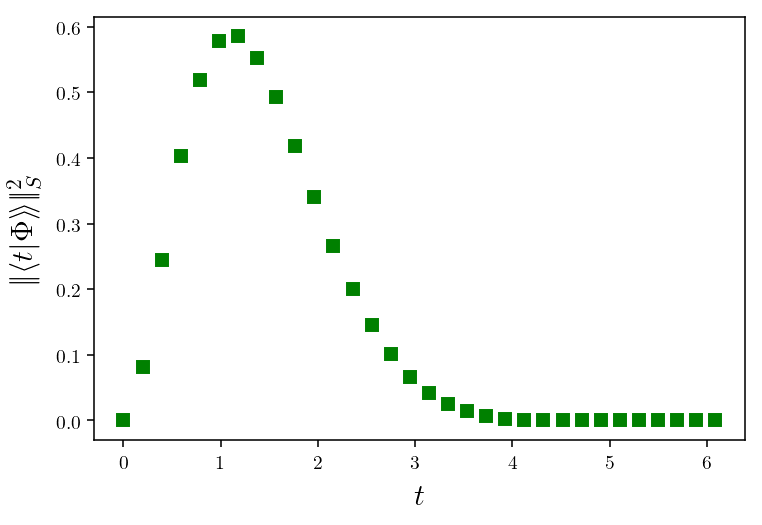
\includegraphics[width=\linewidth]{img/2ldetect/pw-detect-prob.png}
    \subcaption{}\label{fig:2l_pw_detect_prob_t}
  \end{subfigure}
  \begin{subfigure}[b]{0.49\textwidth}
    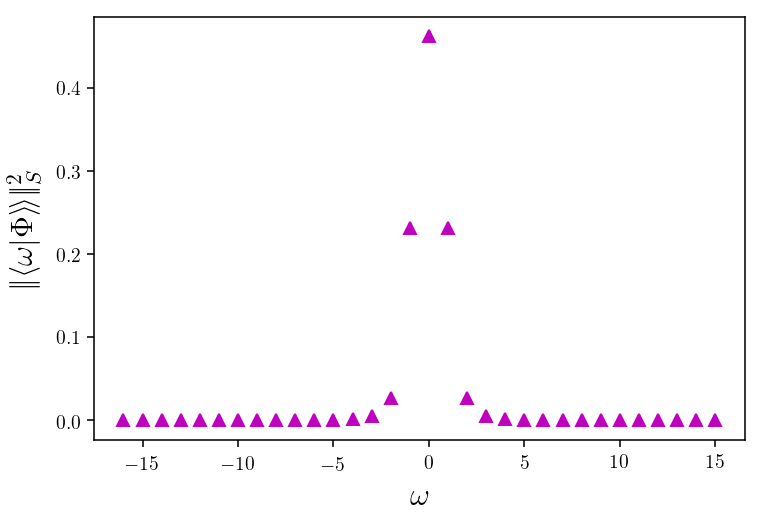
\includegraphics[width=\linewidth]{img/2ldetect/pw-detect-prob-ft.png}
    \subcaption{}\label{fig:2l_pw_detect_prob_omega}
  \end{subfigure}
  \caption{
    Arrival at the detector, probability distribution:
    \subref{fig:2l_pw_detect_prob_t} in the time domain
    and \subref{fig:2l_pw_detect_prob_omega} in the frequency domain.
  }
  \label{fig:2l_pw_detect_prob}
\end{figure}

\subsubsection{Time--energy uncertainty relation}

In quantum systems described by a finite Hilbert space,
uncertainty relations are quantified in terms of \term{entropies}
of the canonically conjugate probability distributions
---see Section \ref{sec:finite_uncertainty} and references therein,
in particular \cite{FiniteHilb}.

In our example, the entropic uncertainty relation explicitly reads:
\begin{multline}
 S_T + S_{\Omega} =
  -\sum_t \norm{\bradket{t}{\Phi}}_S^2 \ln \norm{\bradket{t}{\Phi}}_S^2
  -\sum_{\omega} \norm{\bradket{\omega}{\Phi}}_S^2 \ln \norm{\bradket{\omega}{\Phi}}_S^2 \\
%
  = -\sum_{n=0}^{N-1} \left(\abs{\Phi_{2n}}^2 + \abs{\Phi_{2n+1}}^2\right) \ln \left(\abs{\Phi_{2n}}^2 + \abs{\Phi_{2n+1}}^2\right) \\
    -\sum_{m=0}^{N-1}
          \left(\abs{\tilde{\Phi}_{2m}}^2 + \abs{\tilde{\Phi}_{2m+1}}^2\right)
      \ln \left(\abs{\tilde{\Phi}_{2m}}^2 + \abs{\tilde{\Phi}_{2m+1}}^2\right) \\
%
  \geq \ln N
\end{multline}
---where we had computed previously the probability values in parenthesis.

In Section \ref{jupy:entropic-uncertainties}, we numerically find that
\begin{equation*}
  S_{T} + S_{\Omega} \approx 1.14 \cdot \ln N
\end{equation*}
i.e. circa $14\%$ more than the theoretical minimal uncertainty.

In terms of uncertainty relation based on standard deviations,
which is the standard formulation, particularly for continuous distributions,
and allows a comparison with \cite{RuschhauptAbsorption}, we compute numerically
\begin{equation}\label{eq:uncertainty-us}
  \sigma_{T} \sigma_{\Omega} \approx 0.716 \, \text{,}
\end{equation} \citereset
while \cite{RuschhauptAbsorption} finds
\begin{equation}\label{eq:uncertainty-them}
  \sigma_{T} \sigma_{\Omega} \approx 0.707 \, \text{.}
\end{equation}

It's worth observing that the example in \cite{RuschhauptAbsorption}
sets the optimal parameters to minimize the time--energy uncertainty
\emph{within the given constraints} of the particular physical system,
they don't necessarily achieve the theoretical Heisenberg minimum of
$\frac{\hbar}{2}$
(or $0.5$ in our numerical problem where $\hbar$ has been adimendsionalized).
More notably, parameters therein have been chosen so to minimize
an alternative definition of time--energy uncertainty, $\expval{T}\sigma_E$,
deemed more meaningful within the physics of the particular system.

Nonetheless, with minimal or not minimal uncertainty states (or ``histories''),
a comparison of such uncertainties between the discrete Page--Wooters model implemented
here and the model in \cite{RuschhauptAbsorption} can be performed:
the difference between the results in \eqref{eq:uncertainty-us}
and \eqref{eq:uncertainty-them} may be large enough to be not simply
due to numerical approximation. A further line of investigation
will involve increasing the resolution (number of levels) of the quantum clock:
if the discrepancy persists, an experimental verification
---like those proposed in the paper itself---
will then be of
particular interest.
